% TeX encoding = utf8
% TeX spellcheck = pl_PL 
\documentclass[a4paper, 12pt]{article}
\usepackage[utf8]{inputenc}
\usepackage[polish]{babel}
\usepackage{polski}
\usepackage{graphicx}
\usepackage{url}
\usepackage{caption}
\usepackage{hyperref}
\usepackage[top=2.5cm, bottom=2.5cm, left=3.5cm, right=2.5cm]{geometry}

\begin{document}

\begin{titlepage}
	\begin{center}
		\Large{3 lipca - 11 sierpnia 2017} \\
		[2cm]
		\Huge{\textsc{Praktyki zawodowe}} \\
		\large{\textsc{raport z poczynionyhc prac}}\\ 
		[10cm]
		\Large{Karolina Borkowska}\\ 
		[1cm]
		\large{Opiekun praktyk:}\\
		\Large{mgr inż. Rafał Miśkiewicz}
	\end{center}
\end{titlepage}


\tableofcontents
\newpage

\section{Cel pracy}
Celem pracy jest zaprojektowanie i~zaimplementowanie oprogramowania 
 wykorzystującego płytkę Raspberry Pi jako panel operatorski do zadawania sygnałów układów przekształtnikowych.
\section{Raport postępów pracy}
\subsection{Tydzień pierwszy}
\begin{enumerate}
	\item Zapoznanie się z~dostarczonym sprzętem (płytka Raspberry Pi, moduł rozszerzający DVK512)
	\item Przeanalizowanie potrzeb sprzętowych oraz programowych do komunikacji za pomocą protokołu CAN. Złożenie zamówienia na brakujące moduły.
	\item Zaprojektowanie wstępnej wersji GUI:
		\begin{itemize}
			\item Wybranie języka programowania: \verb|Python 3|
			\item Analiza dostępnych narzędzi i~bibliotek do pracy w~środowisku okienkowym, Wybór platformy programistycznej \verb|Qt| oraz odpowiadającej jej nakładki dla \verb|Python'a| \verb|PyQt5|.
			\item Porównanie dostępnych bibliotek do tworzenia wykresów oraz możliwości zapewnianych przez wyżej wymienioną platformę. W~związku z~nakładem pracy potrzebnej do stworzenia wykresów, które posiadają funkcjonalność rozbudowaną tak samo jak gotowe rozwiązania postanowiono wykorzystać \verb|PyQtGraph|. Jest to narzędzie szybsze od \verb|Matplotlib| (które rozwarzano ze względu na podobieństwo do grafów \verb|Matlab'a|), tworzy rysunki na ciemnym tle (zgodnie z~zaleceniami dla HMI), jest łatwo aplikowalny oraz jest ciągle rozwijane (w przeciwieństwie do np. \verb|GuiQwt|). Jako że nie współpracuje ono z \verb|PyQt5|, zamieniono ją na \verb|PyQt4|.
			\item Implementacja przykładowego wykresu oraz symulacja napływu danych za pomocą \verb|QSlider'a| wywołującego sygnał do aktualizacji wykresu. 
			\item Pobieranie czasu z~systemu oraz wyświetlanie go na osi odciętych.
		\end{itemize}
		Jako, że pamięć urządzenia \verb|Pi| jest znacznie ograniczona, a~praca nad programem jest zwiazana z~instalacją ostatecznie nieużywanych pakietów/programów, prace przeprowadzano na prywatnym komputerze. 
		Wyniki prac przedstawiono na rysunku \ref{fig:win2}.
		\begin{figure}[h!]
			\centering
			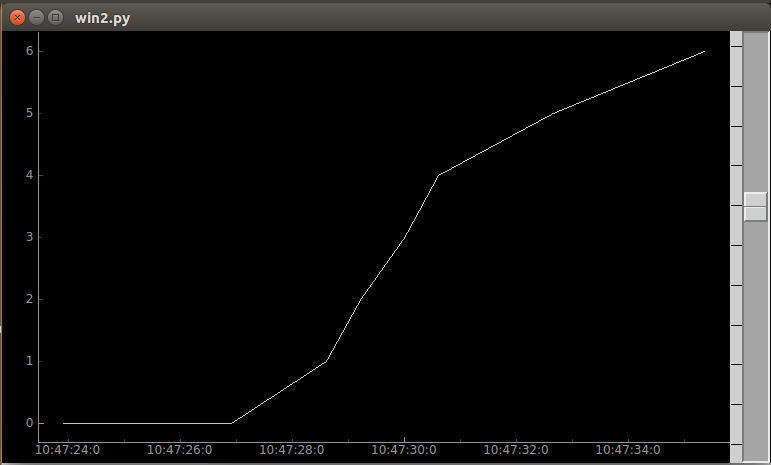
\includegraphics[width=0.8\textwidth]{zdjecia/tydzienuno.png}
			\caption{Prototyp GUI}
			\label{fig:win2}
		\end{figure}
\end{enumerate}
\newpage
\subsection{Tydzień drugi}
\begin{enumerate}
	\item Dodanie milisekund do czasu odczytu danych.
	\item Naprawa wycieku pamięci.
	\item Usunięcie problemu zanikających \verb|QWidget'ów| w~wypadku zmiany wielkości okna oraz nakładającego się na obszar klienta pasa tytułowego okna. 
\end{enumerate}

\end{document}



